\chapter{DWT-SVD增强算法}\label{chap:DWT-SVD}

		\section{奇异值分解算法}奇异值分解最初是由差分几何形成的,希望通过它所作用的两个空间的独立正交变换来确定真正的双线性形式是否可以与另一个形式相等。 Eugenio Beltrami和Camille Jordan分别在1873年和1874年分别发现了双线性形式的奇异值(用矩阵表示)形成了正交替换下双线性形式的一组完整的不变量。詹姆斯约瑟夫西尔维斯特在1889年也得到了实数矩阵的奇异值分解。西尔维斯特将奇异值称为矩阵$A$的正规乘子。第四位独立发现奇异值分解的数学家是1915年的Autonne,他通过极坐标分解到达它。矩阵和复矩阵的奇异值分解的第一个证乎是Carl Eckart和Gale Young于1936年提出的,他们将看作奇异值是Hermitian矩阵主轴变换的推广。1907年,艾哈德施密特为整数算子定义了一个奇异值的类比。似乎他并不知道有限矩阵奇异值的并行工作。计算SVD的实用方法可以追溯到1954年,1955年和1958年Hestenes 。类似于Jacobi特征值算法,它使用平面旋转或Givens旋转。然而,这些被Gene Golub和William Kahan于1965年发表的方法取代,使用Householder变换或反射。 1970年,Golub和Christian Reinsch 发表了Golub / Kahan算法的一个变体,该算法仍然是今天最常用的算法。

SVD定理的几何意义:对于每个线性映射$T:K^n→K^m$,可以找到$Kn$和$Km$的正交基,使得$T$将$Kn$的第$i$个基矢量映射到非负倍$Km$的第$i$个基矢量,并令剩余基矢量为零。

SVD是最小二乘意义下的最优矩阵分解,它将最大信号能量尽可能地分解为尽可能少的系数。奇异值分解(Singular Value Decomposition, SVD)是一种稳定而有效的方法,将系统分解为一组线性无关的分量,每个分量都对系统有一定程度上的贡献。奇异值分解是数值分析中用于对角化矩阵的数值技术。由于SVD具有无穷无尽的优点,如压缩中,在两个独特的子空间数据和噪声子空间的基础上处理图像的能力,所以SVD是一种有吸引力的图像处理代数变换,它通常用于噪声过滤,也被用于水印应用。这些应用程序中的每一个都利用了SVD的关键属性。奇异值分解是鲁棒可靠的正交矩阵分解方法,这是由于其概念和稳定性原因在信号处理领域越来越流行。本文主要介绍奇异值在图像增强的的应用。以下介绍奇异值分解的数学表达。
			\subsection{奇异值分解的数学表达}在线性代数中,SVD是矩阵实数或复数矩阵的分解,类似于使用特征向量的基础的对称或厄密特矩阵的数量化。 SVD是将系统分解为一组线性独立分量的稳定且有效的方法,具有$N \leq M$的尺寸为$M×N$的数字图像$X$可以通过其如下的SVD来表示;
\begin{equation}	\left[ X \right] _{N×M}=\left[ U \right] _{M×M} \left[ S \right] _{M×N} \left[ V \right] ^T_{N×N}	\end{equation}			
\[ U=[u_1,u_2....u_m],	V=[v_1,v_2....v_n] \]
\[
S
=\begin{bmatrix}
s_1  &  0  & \cdots\ &0\\
0  &  s_2  & \cdots\ & 0\\
 \vdots   & \vdots & \ddots  & \vdots  \\
 0 & 0  & \cdots\ & s_n\\
\end{bmatrix}
\]

其中$U$是$M×M$的正交矩阵,$V$是$N×N$的正交矩阵,$S$是$M×N$的矩阵,并且对角元素$s_i$是矩阵$X$的奇异值,下标$T$表示矩阵的转置。正交矩阵$U$的列被称为左奇异向量(Left Singular Vector, LSV),正交矩阵$V$的列被称为右奇异向量(Right Singular Vector, RSV)。$X$的左奇异向量是$XX^T$的特征向量,$X$的右奇异向量是$X^TX$的特征向量。每个奇异值(singular value,SV)指定图像层的亮度,而相应的奇异向量指定图像的几何形状。 U和V是正交矩阵(每列的平方和是独立的,且每个列互不相关),$S$是奇异值递减的对角矩阵。%每个特征图像的奇异值就是它的2-范数。因为SVD使最大奇异值最大化,所以第一特征图像是占最大量的方差 - 协方差结构的模式
		
		\section{小波变换理论}在数值分析和功能分析中,离散小波变换(Discrete Wavelet Transform, DWT)是对任何小波进行离散采样的小波变换。 。小波变换的基本思想是可变窗口的平移和伸缩的基本思想。Haar基是一种最简单的小波基,具有不连续性的特点。小波变换能自动调节频率窗口和时间窗口并能使频域和时域同时进行局部变换,这一特点是小波变换优于傅里叶变换的地方。小波的特点有:长度有限,均值为零。小波变换能够使用伸缩和平移的特性从多个角度细化目标函数。

与小波变换有关的第一个文献是Haar小波。 它是1909年由数学家Alfrd Haar提出的。然而,小波的概念当时并不存在。 直到1981年,这个概念才由地球物理学家让·莫雷特提出。 之后,Morlet和物理学家Alex Grossman在1984年发明了小波项。在1985年之前,Haar小波是人们唯一知道的正交小波。 许多研究人员甚至认为除了Haar小波之外没有正交小波。 此后,数学家Yves Meyer于1985年构造了第二个正交小波Meyer小波。随着越来越多的学者加入这一领域,第一次国际会议于1987年在法国举行。1988年,Stephane Mallat和Meyer提出了多重解决的概念。 同年,Ingrid Daubechies发现了一种构造紧支撑正交小波的系统方法。 1989年,Mallat提出了快速小波变换。 随着这种快速算法的出现,小波变换在信号处理领域有很多应用。
			\subsection{离散小波变换}二维离散小波变换是连续信号离散化后的小波变换,可以用来分析诸如图像的二维离散信号,并在图像压缩领域,数字水印领域,图像融合领域皆有所应用。本文着重强调其在图像增强上的应用。DWT示意图图如下所示:

\begin{figure}[!htbp]
    \centering
    \includegraphics[width=0.40\textwidth]{DWT}
    \bicaption{Q判据等值面图,同时测试一下一个很长的标题,比如这真的是一个很长很长很长很长很长很长很长很长的标题。}{Isocontour of Q criteria, at the same time, this is to test a long title, for instance, this is a really very long very long very long very long very long title.}
    \label{fig:tc_q_criteria}
\end{figure}


%				\begin{figure}[!ht]\centering
%					\includegraphics[totalheight=40mm,width=160mm]{./figures/DWT.jpg}
%					\caption{DWT二级小波变换分解图\label{DWT}}	
%				\end{figure}		

其中,$L$是高低滤波器,$H$是高通滤波器。原始图像经过以及分解后会得到$LL_1$、$HL_1$、$LH_1$、$HH_1$四个子带,子带即一幅图像被分解为一组频带受限的分量,并且子带可以重组在一个构成无误差的原始图像。$LL_1$是水平及垂直方向上的低频子带,$LH_1$是水平方向上低频并且垂直方向上高频的子带,$HL_1$是水平方向上高频并且垂直方向上低频的子带,$HH_1$是水平及垂直方向上都高频的子带。而$LL_2$、$HL_2$、$LH_2$、$HH_2$是子带$LL_1$再次进行一次DWT运算的子带。现在以第一次小波分解为例,进行演示。

\begin{figure}[!htbp]
    \centering
    \begin{subfigure}[b]{0.35\textwidth}
      \includegraphics[width=\textwidth]{LL}
      \caption{}
      \label{fig:oaspl_a}
    \end{subfigure}%
    ~%add desired spacing
    \begin{subfigure}[b]{0.35\textwidth}
      \includegraphics[width=\textwidth]{HL}
      \caption{}
      \label{fig:oaspl_b}
    \end{subfigure}
    \begin{subfigure}[b]{0.35\textwidth}
      \includegraphics[width=\textwidth]{LH}
      \caption{}
      \label{fig:oaspl_c}
    \end{subfigure}%
    ~%add desired spacing
    \begin{subfigure}[b]{0.35\textwidth}
      \includegraphics[width=\textwidth]{HH}
      \caption{}
      \label{fig:oaspl_d}
    \end{subfigure}
    \bicaption{总声压级。(a) 这是子图说明信息,(b) 这是子图说明信息,(c) 这是子图说明信息,(d) 这是子图说明信息。}{OASPL.(a) This is the explanation of subfig, (b) This is the explanation of subfig, (c) This is the explanation of subfig, (d) This is the explanation of subfig.}
    \label{fig:oaspl}
\end{figure}

%				\begin{figure}[ht]
%					\begin{minipage}{0.48\linewidth}
%						\centerline{\includegraphics[width=1\textwidth]{./figures/LL.eps}}
%						\centerline{LL}
%	%				\end{minipage}
%	%				\qquad
%					\begin{minipage}{0.48\linewidth}
%						\centerline{\includegraphics[width=1\textwidth]{./figures/HL.eps}}
%						\centerline{HL}
%					\end{minipage}
%
%					\begin{minipage}{0.48\linewidth}
%						\centerline{\includegraphics[width=1\textwidth]{./figures/LH.eps}}
%						\centerline{LH}
%					\end{minipage}
%					\qquad
%					\begin{minipage}{0.48\linewidth}
%						\centerline{\includegraphics[width=1\textwidth]{./figures/HH.eps}}
%						\centerline{HH}
%					\end{minipage}
%					\caption{DWT示例\label{DWT}}
%				\end{figure}

这里图像的频率指的是图像中灰度变化剧烈强度,是灰度平面上的梯度。图像中的高频分量,指的是图像强度(亮度、灰度)变化剧烈的地方,即边缘(轮廓)以及细节特征。图像中的低频分量,指的是图像强度(亮度、灰度)变换平缓的地方,即大片色块的地方。从图$3.2$中可以看出子带$LL$中包含了原始图像的大部分信息,子带$HL$中主要包含了原始图像的水平方向的轮廓信息,子带$HL$中主要包含了原始图像的垂直方向的轮廓信息,子带$HH$中主要包含了原始图像的轮廓信息及其噪声。以下将展示离散小波变换在保留图像轮廓中的应用。

图$3.3$是子带$HL$、$LH$、$HH$与一个横列分别与子带$LL$相同的零矩阵(即规模相同的全黑矩阵)进行离散小波反变换(IDWT)的结果图,从中可以看出离散小波反变换可以将子带$HL$、$LH$、$HH$还原成一幅保留原始图像大致轮廓的轮廓图。并且用离散小波反变换将子带$LL$、$HL$、$LH$、$HH$还原而成的图像将于原始图像一致,不会有数据丢失。

\begin{figure}[!htbp]
    \centering
    \includegraphics[width=0.40\textwidth]{IDWTWithoutLL}
    \bicaption{Q判据等值面图,同时测试一下一个很长的标题,比如这真的是一个很长很长很长很长很长很长很长很长的标题。}{Isocontour of Q criteria, at the same time, this is to test a long title, for instance, this is a really very long very long very long very long very long title.}
    \label{fig:tc_q_criteria}
\end{figure}

%			\begin{figure}[!ht]\centering
%				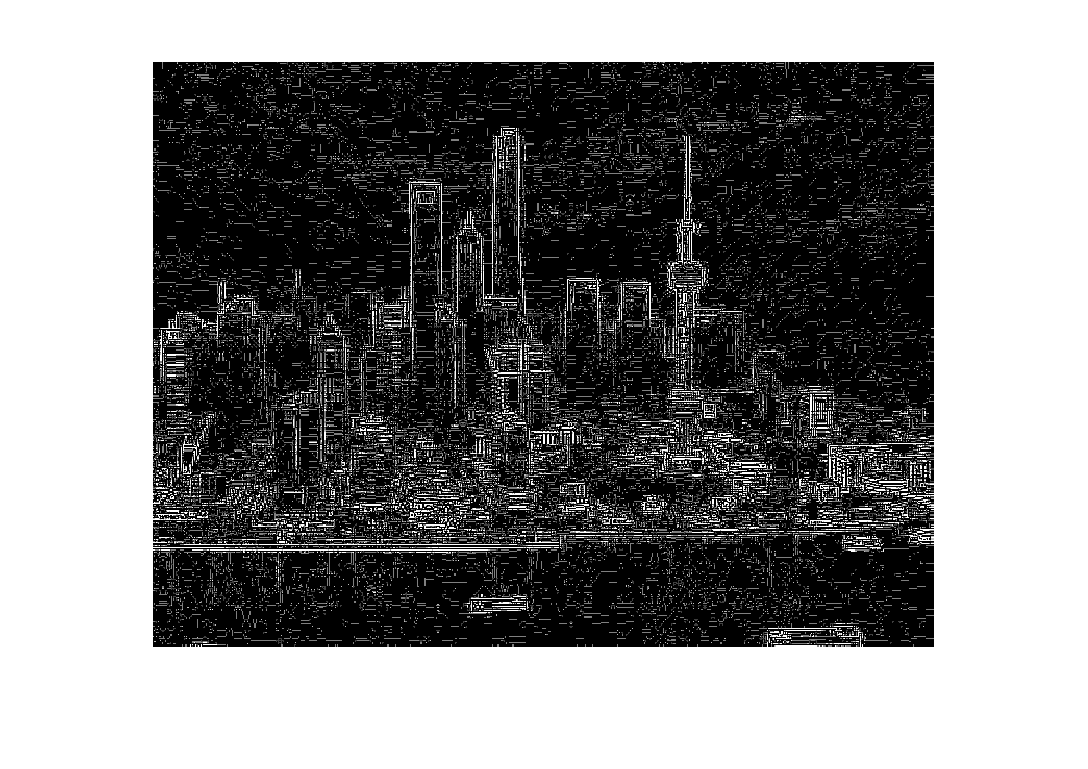
\includegraphics[totalheight=60mm]{./figures/replaceImageLL.eps}
%				\caption{DWT在保留轮廓中的应用\label{DWT}}
%			\end{figure}


	\section{DWT-SVD算法}本文提出的基于DWT-SVD算法的航空图像增强分成为两个部分,第一个部分是使用奇异值分解获得原始图像的奇异值矩阵,改变奇异值矩阵中的数值将会直接影响到图像的亮度并且其余信息保持不变\cite{improved...}。第二部分,是使用直方图均衡,使目标图像的对比度增强。第三部分是使用离散小波变换对原始图像进行处理以保留原始图像的主要轮廓和图像细节,以便进行还原是最终图像有较好的对比度和图像细节。

首先,对输入的灰度航空图像‘$A$’进行直方图均衡处理生成‘$A^*$’,在得到‘$A^*$’后对图像‘$A$’和图像‘$A^*$’进行离散小波变换,分别得到子带$LL$、$HL$、$LH$、$HH$和子带$LL^*$、$HL^*$、$LH^*$、$HH^*$。第二部分别对子带$LL$和$LL^*$进行奇异值分解得到$U_{LL}$、$S_{LL}$、$V_{LL}$和$U_ {LL^*}$、$S_{LL^*}$、$V_{LL^*}$。然后通过下式计算两个奇异值矩阵的相关系数:
\begin{equation}     \xi = \frac{max \left( S_{LL^*} \right) }{ max \left( S_{LL} \right) }    \end{equation}

其中,$S_{LL}$是原始图像$A$的低频系数奇异矩阵,$S_{LL^*}$是原始图像经过直方图均衡化后得到的图像$A^*$的低频系数奇异矩阵。
\begin{equation}     \bar{S}_{LL} = \xi S_{LL}    \end{equation}
\begin{equation}     \bar{LL} =  U_{LL} \bar{S}_{LL} V_{LL} \end{equation}

式$3.2$和式子$3.3$的效果是将使直方图均衡化后的图像‘$A^*$’(或是包含了‘$A^*$’大部分信息的子带$LL^*$)所具有的使图像对比度增强的性质赋予了子带$LL$产生新的子带$\bar{LL}$。式$3.4$中的$\bar{LL}$为低频系数矩阵$S_{LL}$经过奇异值矩阵的相关系数$\xi$增强后再经过奇异值分解公式得到的结果。然后在对进行$\bar{LL}$、$HL$、$LH$、$HH$进行离散小波变换:
\begin{equation}     \bar{A} = IDWT(\bar{LL},HL,LH,HH)    \end{equation}

由于直方图均衡能使图像对比度增强,视觉效果好。离散小波变换能使图像保留原有的轮廓信息和图像细节。然后通过奇异值分解“连接”这两个算法。这样使得了最终图像$\bar{A}$具有更好的视觉效果和更多的轮廓信息,以达到图像增强的效果。以下展示DWT-SVD的算法流程图:

\begin{figure}[!htbp]
    \centering
    \includegraphics[width=0.40\textwidth]{flowChatOfDWTSVD}
    \bicaption{Q判据等值面图,同时测试一下一个很长的标题,比如这真的是一个很长很长很长很长很长很长很长很长的标题。}{Isocontour of Q criteria, at the same time, this is to test a long title, for instance, this is a really very long very long very long very long very long title.}
    \label{fig:tc_q_criteria}
\end{figure}

%			\begin{figure}[!ht]\centering
%				\includegraphics[]{./figures/flowChatOfDWTSVD.jpg}
%				\caption{DWT-SVD的算法流程图\label{DWT}}
%			\end{figure}

以下将展示原始图像经过DWT-SVD算法增强后的结果:


\begin{figure}[!htbp]
    \centering
    \begin{subfigure}[b]{0.35\textwidth}
      \includegraphics[width=\textwidth]{oriImg11}
      \caption{}
      \label{fig:oaspl_a}
    \end{subfigure}%
    ~%add desired spacing
    \begin{subfigure}[b]{0.35\textwidth}
      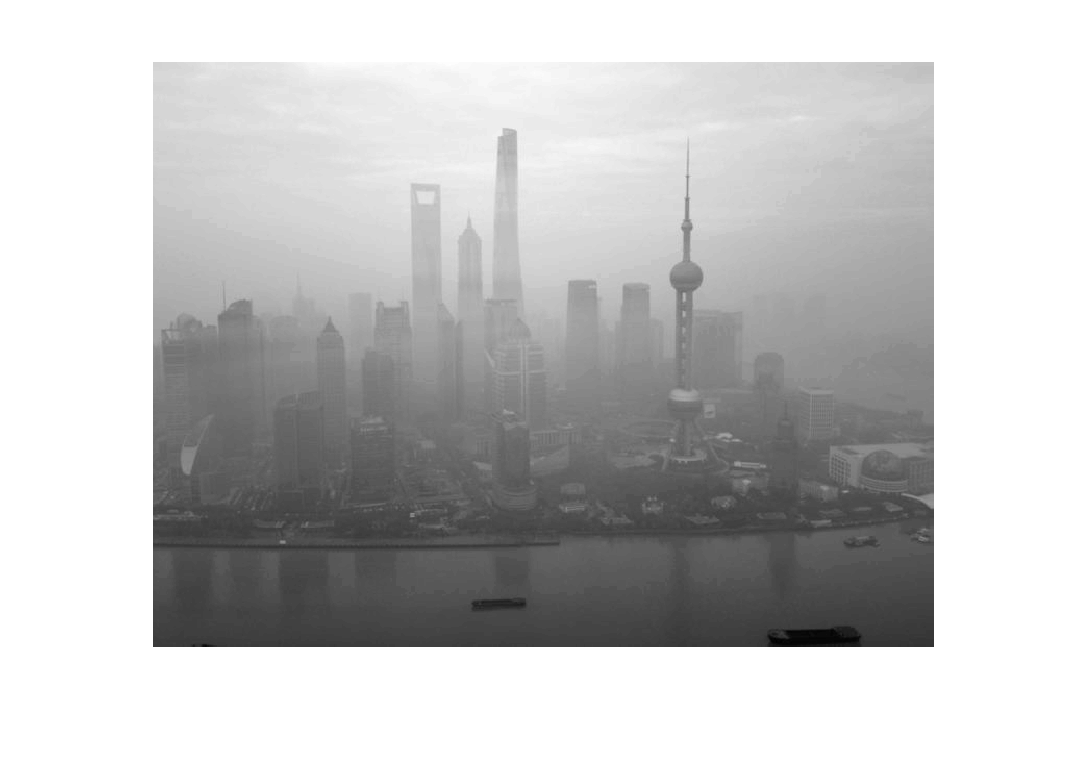
\includegraphics[width=\textwidth]{DWTSVD11}
      \caption{}
      \label{fig:oaspl_b}
    \end{subfigure}
    \bicaption{总声压级。(a) 这是子图说明信息,(b) 这是子图说明信息,(c) 这是子图说明信息,(d) 这是子图说明信息。}{OASPL.(a) This is the explanation of subfig, (b) This is the explanation of subfig, (c) This is the explanation of subfig, (d) This is the explanation of subfig.}
    \label{fig:oaspl}
\end{figure}

%				\begin{figure}[ht]
%					\begin{minipage}{0.48\linewidth}
%						\centerline{\includegraphics[width=1\textwidth]{./figures/originalImage.eps}}
%						\centerline{原始图像}
%					\end{minipage}
%					\qquad
%					\begin{minipage}{0.48\linewidth}
%						\centerline{\includegraphics[width=1\textwidth]{./figures/DWTSVDExample.eps}}
%						\centerline{DWT-SVD增强处理}
%					\end{minipage}
%					\caption{DWT-SVD示例\label{DWT}}
%				\end{figure}

